%%%%%%%%%%%%%%%%%%%%%%%%%%%%%%%%%%%%%%%%%%%%%%%%
% COPYRIGHT: (C) 2012-2015 FAU FabLab and others
% CC-BY-SA 3.0
% EXCEPT for the "Betriebsanweisung" pages!
%%%%%%%%%%%%%%%%%%%%%%%%%%%%%%%%%%%%%%%%%%%%%%%%


\newcommand{\basedir}{fablab-document} % Pfad zur Dokumentenvorlage
\documentclass{\basedir/fablab-document}

\usepackage{booktabs} % für Tabellen: fancy \addlinespace und besondere Querlinien 
\usepackage{pdfpages} % für \includepdf

\usepackage[colorinlistoftodos,prependcaption]{todonotes}
\presetkeys%
    {todonotes}%
    {inline,backgroundcolor=red}{}
\newcommand{\todoUnwichtig}[1]{\textbf{TODO: #1} }
\renewcommand{\texteuro}{\euro}
%\newcommand{\todo}[1]{\textbf{\color{red}{TODO: #1}}}
\newcommand{\pfeil}{\ensuremath{\rightarrow}}
\newcommand{\kommando}[1]{\texttt{#1}}
\newcommand{\tabitem}{~~\llap{\textbullet}~~}
\newcommand{\mcc}[1]{\multicolumn{2}{c}{#1}}
\renewcaptionname{ngerman}{\tablename}{Tab.}
\renewcaptionname{ngerman}{\figurename}{Abb.}

\hyphenation{%
	}

% \linespread{1.2}

%\fancyhead[C]{\textbf{\color{red}{TODO: unfertig!}}}
\date{2015}
\author{kontakt@fablab.fau.de}
\title{Einweisung Ultraschallbad}

\begin{document}
	\maketitle
	
Zur Reinigung von geeigneten Objekten steht ein Emag Emmi-30HC Ultraschallbad zur Verfügung.
Dieses Gerät ist nicht mit Supermarktprodukten niedriger Leistungsklassen zu verwechseln.
Deshalb muss bei der Bedienung auf die folgenden Anweisungen geachtet werden, um Gefährdungen für Mensch und Maschine auszuschließen.
	
\section{Gefahren}
\subsection{Für Benutzer und Umfeld}
Das Ultraschallbad versetzt die darin befindliche Flüssigkeit in starke Schwingungen im Ultraschallbereich und löst somit Verschmutzungen.
Dieser Effekt wirkt auch auf Körperteile, die im Betrieb in Kontakt mit der Flüssigkeit kommen.
\textbf{Es kann somit zu massiven Schädigungen der Knochensubstanz bei Hineinhalten von Körperteilen kommen.}

Durch die eingebaute Heizung und die verhältnismäßig große Querschnittsfläche des Behältnisses wird die Verdampfung des Flüssigkeitsmediums begünstigt.
\textbf{Bei Einsatz von Lösemitteln oder anderen reizenden und oder giftigen Substanzen entstehen reizende und oder giftige Dämpfe.}

Wenn der Hauptschalter auf \enquote{on} steht, kann das Gerät über geringfügige Drehung des Zeitschalters aktiviert werden.
\textbf{Es besteht somit die Gefahr des unbeabsichtigten Einschaltens.}

\subsection{Für das Gerät}
Das Flüssigkeitsgefäß des Ultraschallbades ist nicht beständig gegenüber Säuren und Laugen.
Es darf also nicht mit diesen befüllt werden.

Bei zu geringem Flüssigkeitsspiegel wird der Ultraschallwandler überlastet und zerstört.
Ebenso kann das Bad Schaden nehmen, wenn andere Flüssigkeiten als die in dieser Einweisung aufgeführten,
verwendet werden oder zu reinigende Objekte ohne den Einhängekorb direkt auf dem Boden des Gefäßes liegen.

\section{Regeln und Verwendung}
%TODO optional: Diese Sektion etwas schöner gliedern.
Personen ohne unterschriebene Einweisung dürfen dieses Gerät nicht benutzen, auch nicht unter Anleitung.
Zuerst ist die Einweisung zu unterschreiben.

Gerät bis zur Markierung mit Wasser füllen.
Teile in Einhängekorb legen.
Diesen so in das Gerät einsetzen, dass er nicht auf den Boden aufsetzt.

Nur Wasser und gegebenenfalls Ultraschallreiniger verwenden.
Ersatzweise kann statt Ultraschallreiniger auch Universalreiniger-Konzentrat oder Spülmittel eingesetzt werden.
Andere Stoffe sind nicht erlaubt.
Das heißt weder Lösemittel, Alkohol, noch Säuren, Laugen oder sonstige Zusätze.

Für jegliche Arbeiten (Befüllen, Teile einlegen, und so weiter) den \textbf{roten} Hauptschalter ausschalten.
Der Zeitschalter ist nicht ausreichend.
\textbf{Auf keinen Fall in das Bad greifen, während der Hauptschalter auf \enquote{on} steht!}

Im Betrieb regelmäßig (etwa alle 10 Minuten) nach dem Bad schauen und Füllstand kontrollieren.
Die Heizung nur mit integrierter Zeitschaltuhr verwenden, nicht auf Dauerbetrieb (Zeichen $\infty$).
Deckel aufsetzen, damit fremde Personen nicht hineingreifen.

Empfohlener Aufstellungsort ist rechts vom Waschbecken, da das Gerät keine Spritzer des Ätzbades aushält.

Nach Abschluss Kabel ausstecken.
Wasser nach links hinten ausleeren, sodass es nicht auf die Bedienknöpfe oder den Stromanschluss kommt.
Gerät ausspülen, trockenwischen und in die Schublade zurückräumen.

Der Ultraschallreiniger kostet Geld, siehe Etikett.
Wir bitten außerdem um eine Spende für die Instandhaltung des Ultraschallbades, da es wirklich nicht günstig war.

\subsection{Bedienpanel}

\begin{figure}
\centering
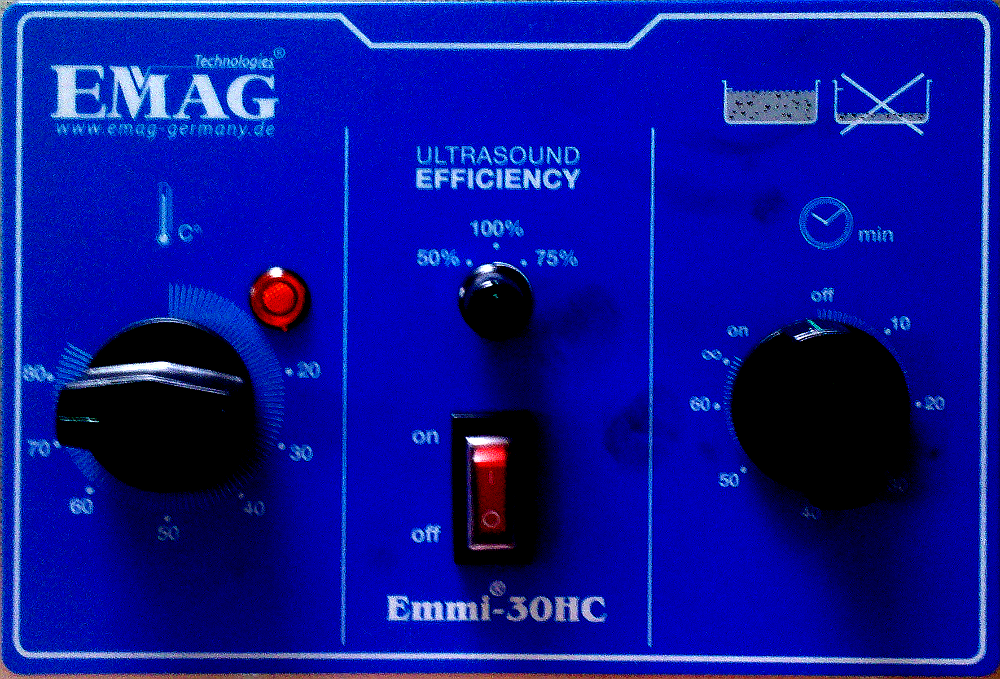
\includegraphics[width=0.6\linewidth]{img/frontpanel.png}
\caption[Abbildung des Bedienpanels]{Abbildung des Bedienpanels}
\end{figure}

Der linke Drehschalter kontrolliert die eingebaute Heizung.
In der obersten Schalterstellung ist die Heizung aus.
Aktivität wird durch die orange-farbene Betriebsleuchte signalisiert.

Der mittlere Drehschalter mit der Aufschrift \enquote{Ultrasound Efficiency} steuert den Tastgrad.
Für den normalen Betrieb ist die Stellung 100 \% gedacht.
In diesem Zustand läuft das Ultraschallbad mit maximaler Leistung.
Die kleineren Tastgrade dienen hauptsächlich zum Einrichten des Bades.

Unter dem mittleren Drehschalter befindet sich der Hauptschalter.
Ausgestattet mit einer Leuchtanzeige zeigt er an, ob das Gerät eingeschalten wurde.
Dieser ist unbedingt auf \enquote{off} zu stellen, bevor in das Bad gegriffen wird.

Der rechte Drehschalter ist der Zeitschalter, welcher den Betriebsmodus einstellt.
Wird der Schalter aus der Grundstellung (\enquote{off}) wenige Grad nach links (in Richtung des $\infty$-Zeichen) gedreht, befindet sich das Bad im Dauerbetrieb.
In diesem Zustand darf die Heizung nicht angeschalten sein.
Wird der Schalter nach rechts gedreht läuft das Bad für die eingestellte Anzahl von Minuten.


\section{Tipps}
Anfangs das Ultraschallbad im Pulsbetrieb (50 \%) verwenden und ab und zu kurz ausschalten, damit sich Luftblasen lösen können.

 \section{Quellen}
  \begin{itemize}
   \item Anleitung Ultraschallbad Emag Emmi-30HC
   \item \href{http://bgi850-0.vur.jedermann.de/index.jsp?isbn=bgi850-0&alias=bgc_bi850_0_bi850_0_s5_2_21_}{BGI 850 5.2.21}
   \item \href{http://www.arbeitssicherheit.de/de/html/library/document/4989034,37}{DGUV Regel 109-010}
  \end{itemize}


\ccLicense{ultraschallbad-einweisung}{Einweisung Ultraschallbad}

\end{document}
